\chapter{Problem Analysis}
\label{cha:Problem Analysis}
\newtext{
Lane merging is not a straightforward problem with a single solution. There are many different types of lane merging scenarios as well as a number of factors which add even more variance. Analysing the different merging scenarios helps to better define the problem and better create solutions for the scenario (\ref{sec:Merge Types}). The factors that could alter the behaviour of a merge scenario should also be defined. This makes it easier to introduce controls in the final simulator which manipulate these factors (\ref{sec:Merge Variance Factors}).
}

\section{Merge Types}
\label{sec:Merge Types}
In this paper we focus on merges made at 'critical positions' such as junctions. This remains constant in all merge types. However, beyond this, there are many different kinds of merge scenarios that a vehicle might encounter.

\subsection{Single-to-Single Merge}
\label{subsec:Single-to-Single Merge}
A single-to-single merge (S2S merge) describes a situation where a vehicle moves from a single lane road into another single lane road, as seen in Figure \ref{fig:S2SMerge}. In this situation we label the lane that vehicles are moving from the 'current lane' (CL), and we label the lane that vehicles move to the 'target lane' (TL). We describe the vehicles that start on the CL as 'merging vehicles' (MV) and the vehicles that start on the TL as 'target vehicles' (TV). We have our critical position where the CL and TL connect. We call the area in which the vehicles in the two lanes merge together our 'merge zone'.

\begin{figure}[htb]
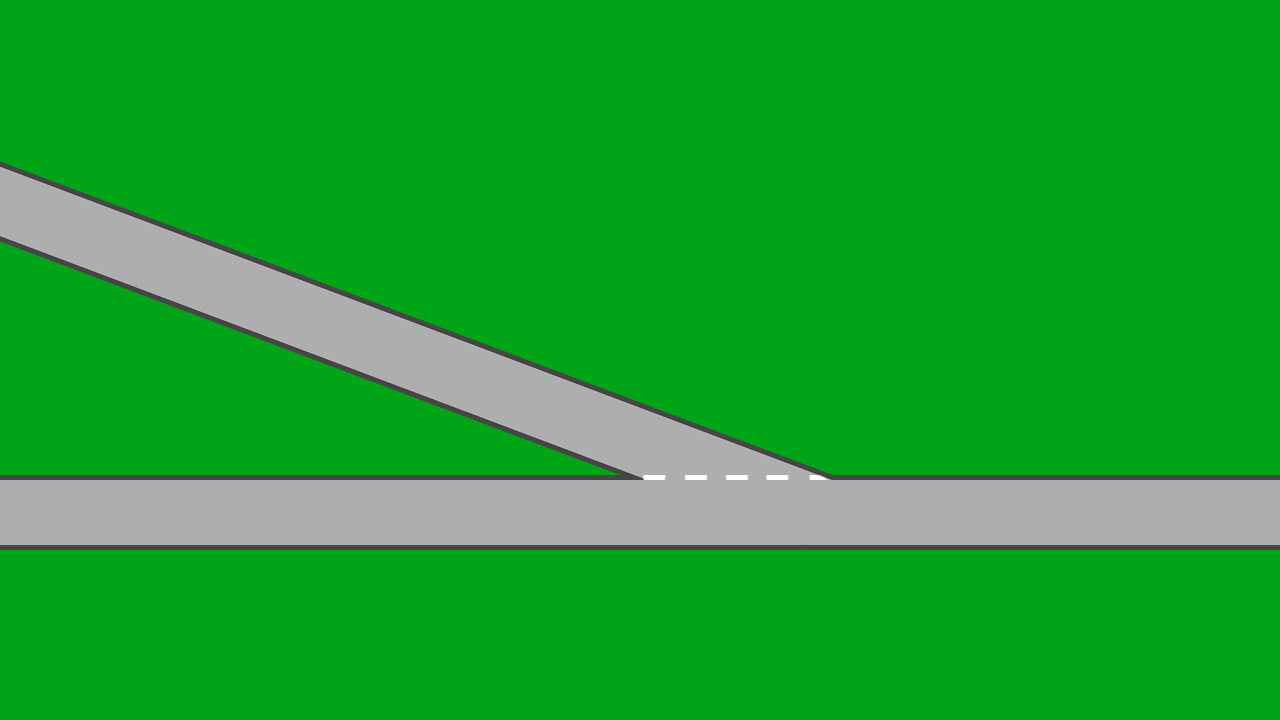
\includegraphics[width=\textwidth]{laneDiagrams/s2s.png}
\caption{A road with a single-to-single lane merge (S2S)}
\label{fig:S2SMerge}
\end{figure}

The main issue with an S2S merge stems from the limited options available to vehicles arriving at the critical position. Target vehicles do not have the opportunity to move laterally out of the way of merging vehicles, and vehicles on both lanes could struggle to reduce their velocity without affecting their successors.

\subsection{Single-to-Single Merge with slip-road}
\label{subsec:Single-to-Single Merge with slip-road}
Many S2S merges are performed with an attached slip-road, as seen in Figure \ref{fig:S2SMergeExtended}. Figure \ref{fig:realLaneMerge} shows a real world single to triple lane merge with a slip-road.

\begin{figure}[htb]{}
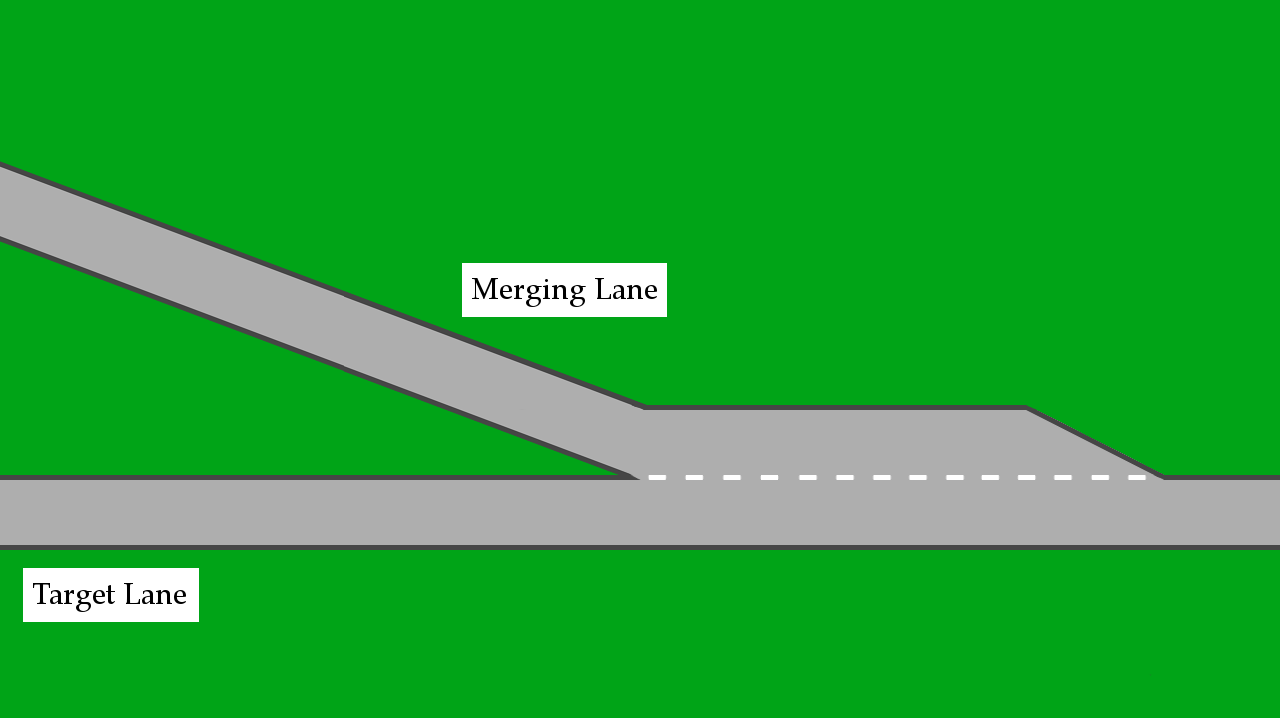
\includegraphics[width=\textwidth]{laneDiagrams/s2sExtended.png}
\caption{A road with a single-to-single lane merge and slip-lane (S2S)}
\label{fig:S2SMergeExtended}
\end{figure}

\begin{figure}[htb]
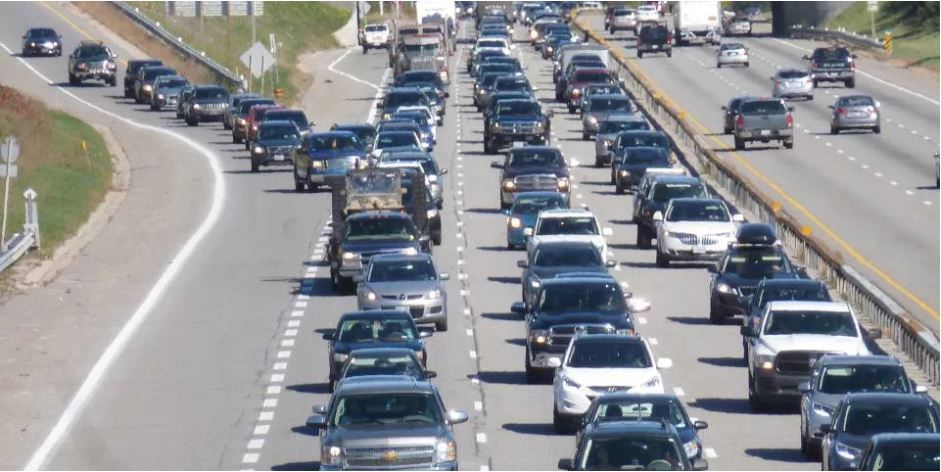
\includegraphics[width=\textwidth]{images/laneDiagrams/realLaneMerge.jpg}
\caption{A real world single to triple lane merge with a slip-road. Image Copyright Nigel Cox. This work is licensed under the Creative Commons Attribution-Share Alike 2.0 Generic Licence. http://creativecommons.org/licenses/by-sa/2.0/ \todo{Lilian, does this mean that I have to share my essay under Creative Commons? If so should I choose a different image?}\citep{realLaneMerge}}
\label{fig:realLaneMerge}
\end{figure}

The slip-road gives merging vehicles more time to travel parallel to the target lane before merging. This makes the merge easier for both MVs and TVs as MVs don't slow down in front of TVs in order to make the turn into the TL. The effectiveness of slip-roads should change with length: the longer the slip-road, the more time MVs have to merge. This should improve the effectiveness of the merge position.

\subsection{Single-to-Double Merge}
\label{subsec:Single-to-Double Merge}
A single-to-double merge (S2D merge) describes a situation where a vehicle moves from a single lane road into a double lane road, as seen in Figure \ref{fig:S2DMerge}. In this situation we have two target lanes. The upper lane which directly links to the merging lane is called 'target lane 1' (TL1) and the lower lane is called 'target lane 2' (TL2). We still have only one critical position where the merging lane meets TL1.

\begin{figure}[htb]
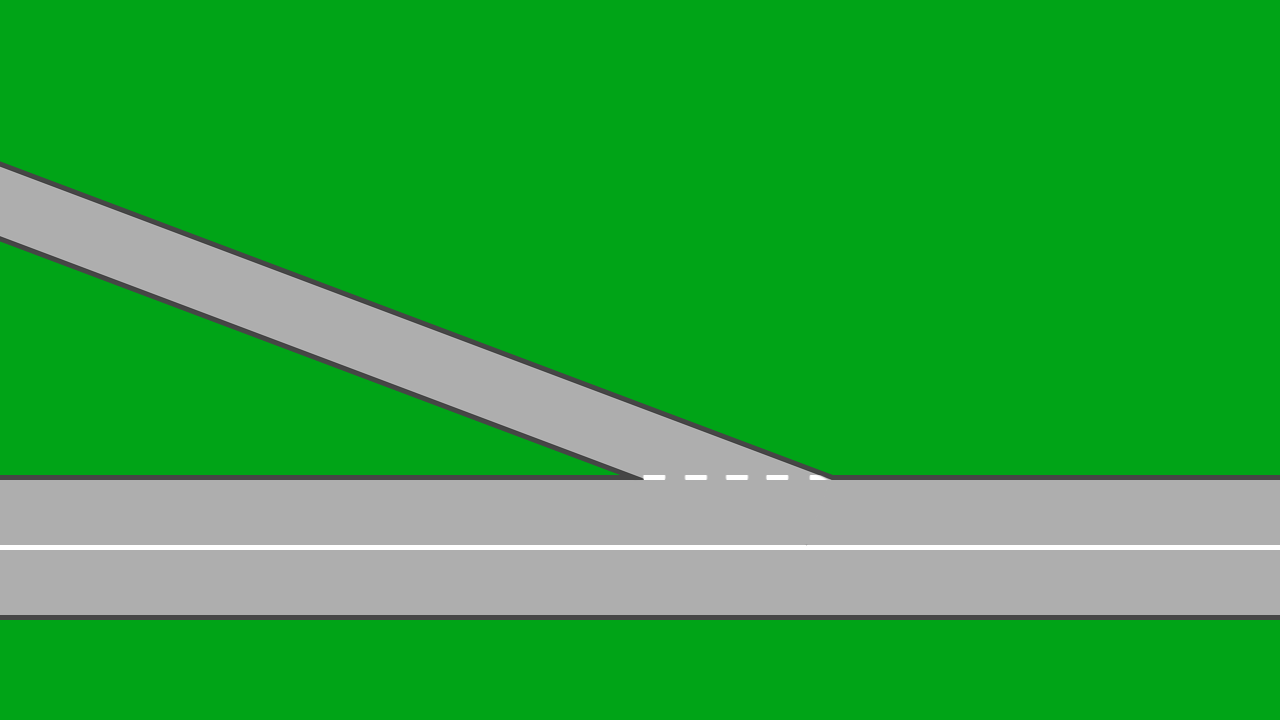
\includegraphics[width=\textwidth]{laneDiagrams/s2d.png}
\caption{A road with a single-to-double lane merge (S2D)}
\label{fig:S2DMerge}
\end{figure}

An S2D merge provides more options for vehicles on the targets lanes at the critical position. Target vehicles now have the opportunity to move laterally to avoid merging vehicles. Two lanes also allows for more vehicles on the target lane which should give vehicles greater freedom to adjust their velocity without affecting their successors, at least when compared to the same number of vehicles on a single lane.

\subsection{Single-to-Double Merge with slip-road}
\label{subsec:Single-to-Double Merge with slip-road}

S2D merges can also take advantage of a slip-road, as seen in Figure \ref{fig:S2DMergeExtended}.

\begin{figure}[htb]
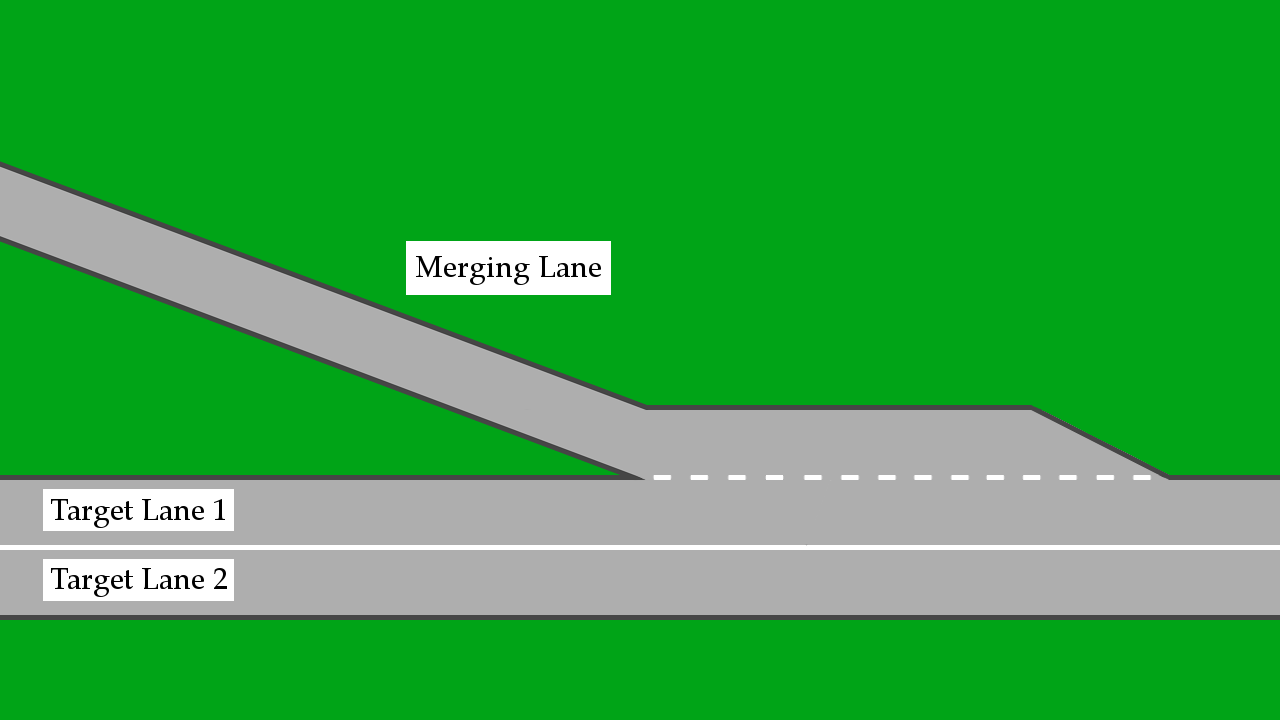
\includegraphics[width=\textwidth]{laneDiagrams/s2dExtended.png}
\caption{A road with a single-to{}-double lane merge and slip-lane (S2D)}
\label{fig:S2DMergeExtended}
\end{figure}

\subsection{Double-to-Double Merge}
\label{subsec:Double-to-Double Merge}
A double-to-double merge (D2D merge) describes a situation where a vehicle moves from a double lane road into another double lane road, as seen in Figure \ref{fig:D2DMerge}. We now have two merging lanes. The upper lane, 'merging lane 1' (ML1) merges into TL1 and the lower lane, 'merging lane 2' (ML2) merges into TL2.

\begin{figure}[htb]
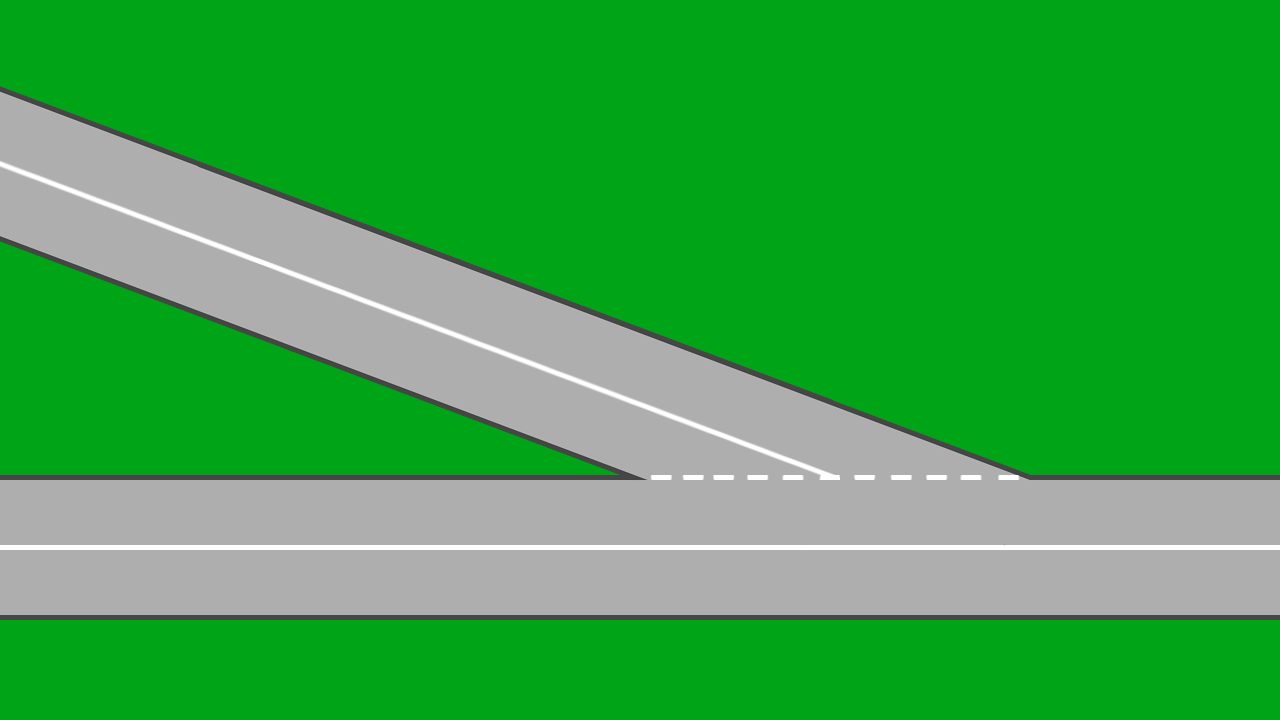
\includegraphics[width=\textwidth]{laneDiagrams/d2d.png}
\caption{A road with a double-to-double lane merge (D2D)}
\label{fig:D2DMerge}
\end{figure}

With a D2D merge we now have to consider the effect of merging vehicles from ML2 driving across TL1. In addition, target vehicles can no longer laterally move out of the way of merging vehicles as they did before. Combining these factors with the wider range of options available to MVs, we can see that a D2D merge is far more complex than an S2D merge.

\subsection{Double-to-Double Merge with slip-road}
\label{subsec:Double-to-Double Merge with slip-road}

D2D merges can also take advantage of a slip-road, as seen in Figure \ref{fig:D2DMergeExtended}.

\begin{figure}[htb]
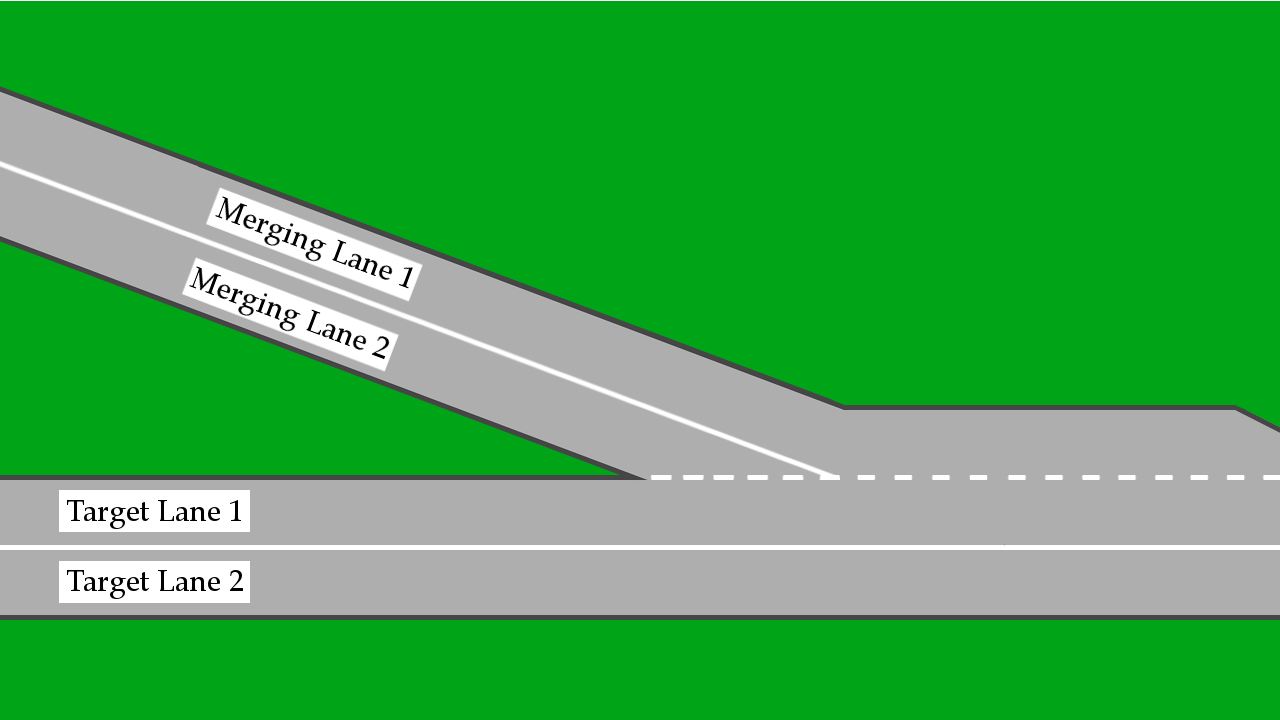
\includegraphics[width=\textwidth]{laneDiagrams/d2dExtended.png}
\caption{A road with a single-to-double lane merge and slip-lane (S2D)}
\label{fig:D2DMergeExtended}
\end{figure}

D2D merges with a slip-road work differently to other slip-road schemes. In this instance vehicles on ML1 and ML2 will both merge into TL1. However, ML2 merges into TL1 as vehicles on an S2D merge would. ML1 vehicles merge into TL1 as vehicles on an S2D merge would when there is a slip-road in play.

\subsection{Lane Obstruction Merge}
\label{subsec:Lane Obstruction Merge}
A lane obstruction merge is where a vehicle needs to change lanes to avoid an obstacle in their way, as seen in Figure \ref{fig:LaneObstruction}. It is essentially an S2S merge although the vehicle will tend to move laterally to avoid the obstacle. In this situation the critical position is a point shortly before the obstruction on the CL. 

\begin{figure}[htb]
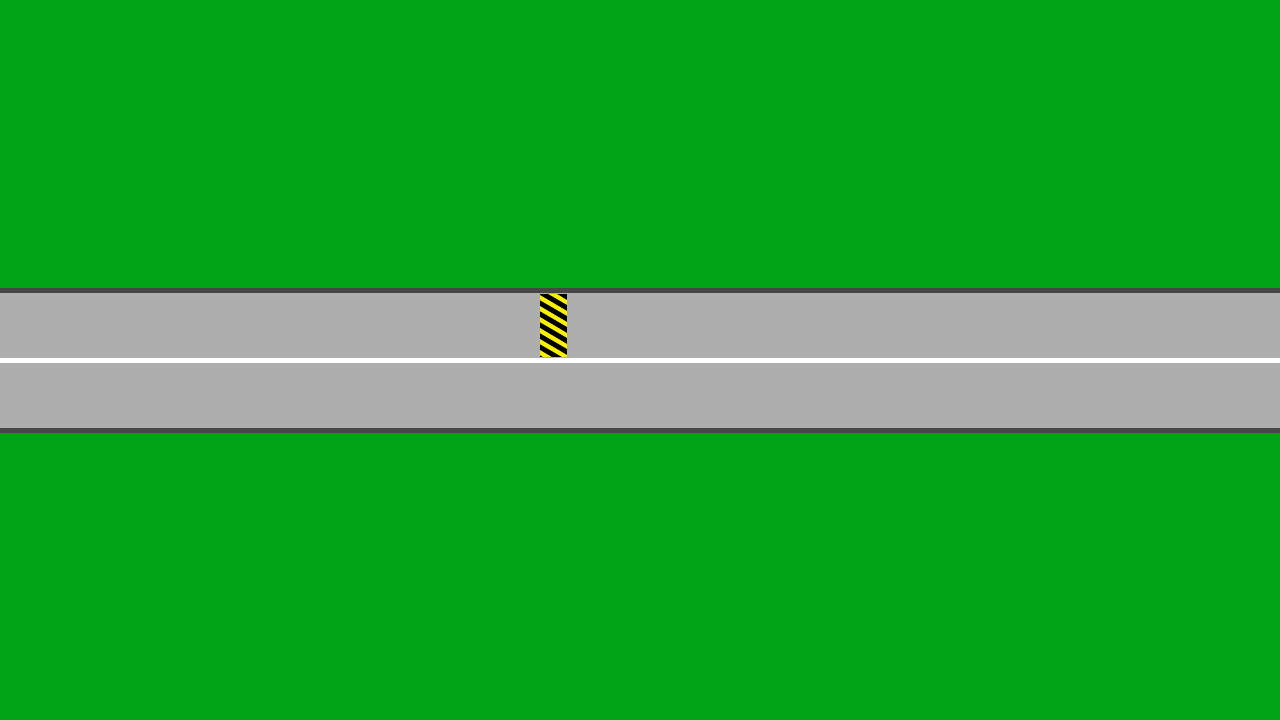
\includegraphics[width=\textwidth]{laneDiagrams/lane_blocker.png}
\caption{A road with a lane obstruction}
\label{fig:LaneObstruction}
\end{figure}

The obstacle could be a broken down vehicle or some debris on the road. Because of the unexpected nature of the obstacle it may sometimes be difficult to have a centralised approach to the problem. Although, if the obstacle was a broken down vehicle, the vehicle might be able to act as the centralised system managing approaching vehicles. 

\section{Measuring Success}
\label{sec:Measuring Success}
In order to evaluate the effectiveness of solutions to the problems we need to define measurements of success. 

Solutions to the merging problems above have to satisfy the following conditions:

\begin{enumerate}
\item \textit{No collisions}
This means avoiding collisions at the critical position between merging vehicles and target vehicles, as well as avoiding collisions between vehicles on the same lane.
\item \textit{Minimise delays to both lanes}
Vehicles should not suffer large delays to travel time due to the merge. This means measuring both average delay and maximum delay. We do not want vehicles on one lane starving (not moving) for the benefit of vehicles on the other lane.
\item \textit{Maximise throughput}
By minimising delays and velocity loss we aim to maximise the throughput of the critical position.
\item \textit{Minimise changes in velocity}
Though not necessary, we should aim to minimises changes in vehicle velocity, for both passenger comfort and vehicle efficiency.
\end{enumerate}

We need to measure how well solutions meet these conditions. 

\subsection{Collisions}
\label{subsec:Collisions}
Preventing collisions is a basic safety requirement for any autonomous vehicle system. We can measure this by comparing the positions of vehicles in the system, and ensuring that there is no overlap.

We should also consider measuring near misses. We can define a minimum spacing between vehicles, perhaps equal to the minimum braking distance of the vehicle plus an additional comfort distance. This would mimic the IDM model \citep{Treiber2000}.

Any collisions that do happen should be reported immediately. The system should automatically be considered a failure.

\subsection{Delay}
\label{subsec:Delay}
Delay measures the effect that the critical position had on the overall journey of the vehicle. It is the primary metric considered in Dresner et al.'s 2004 paper \citep{Dresner2004} on AIM. We will measure delay in a similar manner, calculating both average delay and maximum delay.

Dresner et al. provide the following equation for measuring average delay.

\begin{equation}
\frac{1}{|C|}\sum_{v_i\in{C}}\bigl(t(i) - t_0(i)\bigr)
\end{equation}

$C$ is the set of vehicles that pass through a critical position within a set time frame. Assuming no other vehicles on the road, a vehicle $v_i$ would complete it's trip in time $t_0(i)$, otherwise $v_i$ would complete it's trip in time $t(i)$. We can represent this trip for vehicles in the simulator as the time difference between the vehicle spawning in and the vehicle being removed from the simulator.

Dresner et al. also provide the following equation for measuring maximum worst case delay:

\begin{equation}
\max_{v_i\in{C}}\bigl({t(i)} - t_0(i)\bigr)
\end{equation}

Measuring maximum delay (and minimising it) is important, as we do not want to have a solution where some vehicles have extremely large delay times and others have very low delay times. This should help avoid a 'starvation' situation where some vehicles never get to complete their trips.

\subsection{Throughput}
\label{subsec:Throughput}
By minimising delay we should also maximise throughput; the two are closely related. However we should also collect direct metrics.

\begin{equation}
\text{Vehicle throughput} = \frac{|C|}{t}
\end{equation}

Here $t$ is the time it took for all of the vehicles in $C$ to pass through the critical position. If we want to measure the rate at which merging vehicles and target vehicles pass through the intersection separately we can change the definition of $C$ to reflect that.

\subsection{Velocity Changes}
\label{subsec:Velocity Changes}
Vehicles should aim want to reduce velocity changes as much as possible, aiming especially to eliminate rapid changes. Ideally autonomous vehicles should have very smooth acceleration and braking profiles. This both increases passenger comfort and improves fuel efficiency.

To measure maximum acceleration and deceleration we can assume a constant acceleration/deceleration between the point at which a vehicle decides to start changing velocity and the point at which the vehicle has either reached it's target speed or made a new decision. We can use the time gap between those two points, and the change in the vehicle's velocity, to calculate it's acceleration or deceleration. We then take the maximum values of the acceleration of the vehicle and the deceleration of the vehicle.

\section{Merge Variance Factors}
\label{sec:Merge Variance Factors}
\newtext{ALL NEW TEXT BELOW}

In each of the scenarios in section \ref{sec:Merge Types} the road layout is fixed. More variance can be introduced to the scenarios by altering other factors. Not all of the factors below will be applicable in every merge scenario. Figure \ref{fig:s2sMarked} shows some of the factors below, applied to an S2S merge.

\begin{itemize}
\item \textit{Traffic Level} 
The traffic level changes the number of vehicles on the road at any one time. Effectively, it is used to measure traffic density.
\item \textit{Target lane speed limit}
The maximum speed that vehicles on the target lane can travel.
\item \textit{Merge lane speed limit}
The maximum speed that vehicles on the merge lane can travel.
\item \textit{Target lane lead in distance}
The distance between the point at which target vehicles start being able to make decisions regarding the merge, and the point at which the target vehicles reach the merge zone.
\item \textit{Target lane lead out distance}
The distance between the end of the merge zone and the end of the target lane (at least the end in the simulator).
\item \textit{Merge lane lead in distance}
The distance between the point at which merging vehicles start being able to make decisions regarding the merge, and the point at which the merging vehicles reach the merge zone.
\item \textit{Merging angle}
The interior angle $\theta$ at the point where the merging lane meets the target lane.
\item \textit{Slip-road length}
The length of the slip-road in a merge that uses a slip-road.
\end{itemize}

\begin{figure}[htb]
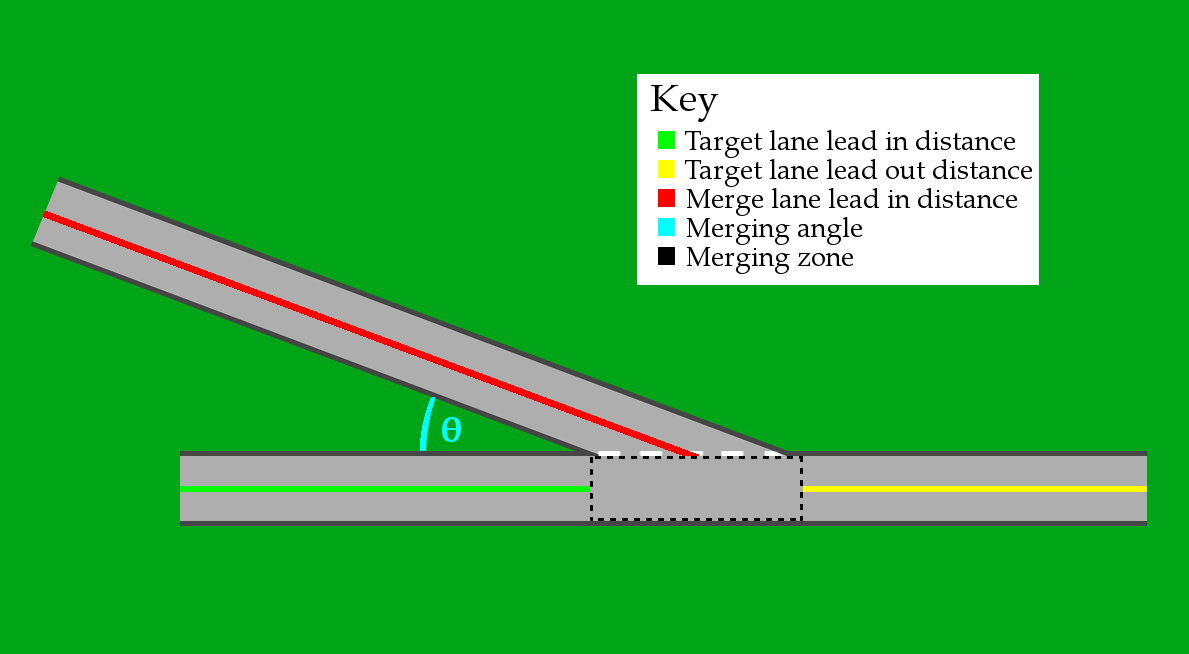
\includegraphics[width=\textwidth]{laneDiagrams/s2sMarked.png}
\caption{An S2S merge marked with some of the variable factors}
\label{fig:s2sMarked}
\end{figure}

Traffic level has a fairly obvious effect on performance in a particular merge scenario. The more vehicles that try to merge together the more difficult it will be for the merge to happen. It will likely require vehicles to be moving much more slowly. Increased traffic density also increases the likelihood of traffic shocks, and vehicle manoeuvrability is impacted.

Altering speed limits also affects performance. Higher speed limits allow vehicles to travel more quickly through the critical position and could improve performance. However, larger speed limits could also lead to larger deceleration and acceleration values. Problems could also arise if there are big differences between the speed limits of the merging lane and target lane. If the target lane speed limit is larger, merging vehicles will slow down target lane vehicles as they merge in. If the merging lane speed limit is larger then merging vehicles may have to declerate quickly to allow target vehicles to move through the merging zone.

Lead in distances change the amount of deliberation time vehicles have before they reach the junction. It also changes the distance they have to change their velocity in. This means that shorter distances could lead to larger acceleration and deceleration values as well as sub-optimal solutions to the merge.

The lead out distance will mostly affect the result collected as the vehicle leaves the simulator. Longer lead out distances allow vehicles to return to their preferred speed. This should give more accurate results for a vehicle's maximum acceleration and deceleration. 

The merging angle changes the length of the merge zone. Shallower angles will lead to longer merge zones due to the width of the merging lane. Shallower merging angles also reduce the turning angle for merging vehicles. This could lead to faster merges as merging vehicles have to make smaller changes to their heading.

\section{Requirements}
\label{sec:Requirements}
By using the problem analysis above we can define requirements for our final system. This system will not deal with every merge scenario described but will instead set the groundwork for further research.

\subsection{Functional}
\label{subsec:Functional}
The functional requirements describe the functionality required within the simulator. They are broken into two sets of requirements. User requirements and system requirements. User requirements describe the behaviour expected from the simulator from a user perspective. System requirements are all associated with a user requirement. They describe the functionality required by the system in order to satisfy the user requirement. Table \ref{tab:functionalRequirements} shows all of the functional requirements.

\begin{longtable}{|p{0.1\linewidth}|p{0.4\linewidth}|p{0.1\linewidth}|p{0.4\linewidth}|}
% Headings and Footers %
\caption{Functional requirements table.}\label{tab:functionalRequirements}\\
\hline
\multicolumn{2}{|l|}{User Requirements} & \multicolumn{2}{l|}{System Requirements} \\
\hline
\endfirsthead

\hline
\multicolumn{2}{|l|}{User Requirements} & \multicolumn{2}{l|}{System Requirements} \\
\hline
\endhead

\hline
\endfoot

\hline
\endlastfoot

% Data %
\multirow{3}{*}{FU.1} & \multirow{3}{*}{\parbox{\linewidth}{Users can run merge simulations.}} 
 & FS.11 & The system has controls for starting merge simulations \\
 &  & FS.12 & The system can create merge simulations \\
 &  & FS.13 & The system can run merge simulations \\
\hline
\multirow{2}{*}{FU.2} & \multirow{2}{*}{\parbox{\linewidth}{User can manipulate the running speed of a simulation.}}
 & FS.21 & The system has controls changing the speed of running simulations. \\
 &  & FS.22 & Merge simulations can have their run speed changed. \\ 
\hline
\multirow{2}{*}{FU.3} & \multirow{2}{*}{\parbox{\linewidth}{User can pause simulations.}}
 & FS.31 & The system has controls allowing running simulations to pause. \\
 &  & FS.32 & Merge simulations can be paused \\ 
\hline
\multirow{2}{*}{FU.4} & \multirow{2}{*}{\parbox{\linewidth}{User can end a simulation.}}
 & FS.41 & The system has controls ending simulations. \\
 &  & FS.42 & Merge simulations can be ended. \\ 
\hline
FU.5 & User can view the activities of a simulation. & FS.51 & The system displays the current status of a simulation as it runs. \\
\hline
\multirow{9}{*}{FU.6} & \multirow{9}{*}{\parbox{\linewidth}{Users can export the results of a merge simulation.}}
 & FS.61 & The system has controls for exporting results data. \\
 & FS.62 & The system can produce a file containing results data from the simulation. \\
 &  & FS.63 & The results file contains the total throughput of the simulation. \\
 &  & FS.64 & The results file contains the maximum delay of the simulation. \\
 &  & FS.65 & The results file contains the average delay of the simulation. \\
 &  & FS.66 & The results file contains the maximum acceleration of the simulation. \\
 &  & FS.67 & The results file contains the maximum deceleration of the simulation. \\
 &  & FS.68 & The results file contains the delay for each vehicle in the simulation. \\
 &  & FS.69 & The results file contains the maximum acceleration for each vehicle in the simulation. \\
 &  & FS.6a & The results file contains the maximum deceleration for each vehicle in the simulation. \\ 
\hline
\multirow{3}{*}{FU.7} & \multirow{3}{*}{\parbox{\linewidth}{Users can select and run an S2S merge simulation.}}
 & FS.71 & The system can produce S2S simulations. \\
 &  & FS.72 & The system has controls allowing S2S simulations to be selected. \\
 &  & FS.73 & The system can run S2S simulations \\ 
\hline
\multirow{2}{*}{FU.8} & \multirow{2}{*}{\parbox{\linewidth}{Users can select a centralised merging scheme with S2S merge simulations.}}
 & FS.81 & The system can use an AIM-like merge management system for the merging zone in an S2S simulation. \\
 &  & FS.82 & The system has controls allowing users to select the merge scheme indicated in FS.71. \\ 
\hline
\multirow{2}{*}{FU.9} & \multirow{2}{*}{\parbox{\linewidth}{Users can select a decentralised merging scheme with S2S merge simulations.}}
 & FS.91 & The system can use an merge management scheme similar to that described in \citep{VanMiddlesworth2008}. \\
 &  & FS.92 & The system has controls allowing users to select the merge scheme indicated in FS.81. \\ 
\hline
FU.10 & Users can control the traffic level of an S2S simulation. & FS.101 & The system has controls for adjusting the traffic for an S2S simulation. \\ 
\hline
FU.11 & Users can control the target lane speed limit of an S2S simulation. & FS.111 & The system has controls for adjusting the target lane speed limit for an S2S simulation. \\ 
\hline
FU.12 & Users can control the merge lane speed limit of an S2S simulation. & FS.121 & The system has controls for adjusting the merge lane speed limit for an S2S simulation. \\ 
\hline
FU.13 & Users can control the target lane lead in distance of an S2S simulation. & FS.131 & The system has controls for adjusting the target lane lead in distance for an S2S simulation. \\ 
\hline
FU.14 & Users can control the target lane lead out distance of an S2S simulation. & FS.141 & The system has controls for adjusting the target lane lead out distance for an S2S simulation. \\ 
\hline
FU.15 & Users can control the merge lane lead in distance of an S2S simulation. & FS.151 & The system has controls for adjusting the merge lane lead in distance for an S2S simulation. \\ 
\hline
FU.16 & Users can control the merge angle of an S2S simulation. & FS.161 & The system has controls for adjusting the merge angle for an S2S simulation. \\ 
\hline
\multirow{2}{*}{FU.17} & \multirow{2}{*}{\parbox{\linewidth}{Users should be alerted of any collisions during a simulation.}}
 & FS.171 & The system should be able to alert the user if a collision occurs. \\
 &  & FS.172 & The simulation should detect collisions. \\ 
\end{longtable}

\subsection{Non-functional}
\label{subsec:Non-functional}
The non-functional requirements describe the expectations of the simulator that are not actions the simulator will perform. Table \ref{tab:nonFunctionalRequirements} shows the non-functional requirements for the simulator.

\begin{longtable}{|p{0.1\linewidth}|p{0.9\linewidth}|}
% Headings and footers %
\caption{Non-functional requirements table.}\label{tab:nonFunctionalRequirements}\\
\hline
ID & Description \\
\hline
\endfirsthead

\hline
ID & Description \\
\hline
\endhead

\hline
\endfoot

\hline
\endlastfoot

% Data %
NS.1 & All system controls come from standard JComponents. \\
NS.2 & All controls are clearly labeled. \\
NS.3 & Simulation creation should take no longer than 3 seconds. \\
NS.4 & Simulations should be able to run faster than real-time. \\
NS.5 & Simulations should update the GUI frequently. \\
NS.6 & All data displayed to the user should be accurate. \\
NS.7 & All data in the results file should be accurate. \\
NS.8 & Created simulators should accurately represent their merge scenario with the provided modifier factors. \\
NS.9 & Code should be written to allow for easy expansion. \\
NS.10 & Code should be well documented. \\
NS.11 & The simulator should be integrated into the AIM4 simulator without negatively affecting the performance of AIM simulations. \\
NS.12 & It should be easy to add new simulator types in AIM4 alongside AIM and Merge simulations. \\
\end{longtable}